\chapter{Dos conceitos principais}
\label{cap:main-concepts}
\minitoc

\intro{Nesse capítulo, o objetivo é explicitar os conceitos que serão cruciais
para a compreensão do que é dito nos demais capítulos. Como já dito, funciona
como o cabeçalho de um arquivo de código em que se inclui as bibliotecas e
demais arquivos com definições e módulos e classes e tudo o mais. Tratando desse
trabalho, é o capítulo que garante que o texto estará auto contido na medida do
possível, ou seja, qualquer um que lê-lo, compreenderá o que estiver escrito sem
ter que pesquisar muito fora daqui.}

\section{O projeto e os conceitos associados}
\label{sec:project}

\subsection{Sobre o NEHiLP e o DELPo}
\label{subsec:nehilp-delpo}

Uma das finalidades principais do NEHiLP é pesquisar sobre Linguística Histórica,
Filologia e Etimologia. Para a pesquisa, requere-se a análise de documentos das
mais variadas épocas, a fim de recolher informações linguísticas. Gerar e organizar
dados para o estudo da história da língua portuguesa é uma das principais metas
deste trabalho.

Nos dias de hoje, o núcleo de pesquisa conta com projetos associados a diferentes
universidades. Estes projetos são: \begin{itemize}
   \item \href{https://gruponemesis.ufba.br/projetos/dicion\%C3\%A1rio-dialetal-brasileiro}{DBB},
   \href{https://gruponemesis.ufba.br/projetos/dicion\%C3\%A1rio-etimol\%C3\%B3gico-do-portugu\%C3\%AAs-arcaico}{DEPARC}
   \footnote{vinculados a UFBA}
   \item LIBOLO \footnote{vinculado a Macau University e USP}
   \item \href{http://ccint.fflch.usp.br/projeto-de-historia-do-portugues-paulista-phpp-projeto-caipira-2}{PHPP} \footnote{vinculado a UNESP e USP}
   \item MAP (Mulheres na América Portuguesa) \footnote{vinculados a USP}
   \item DELPo -- centro da atenção nesse trabalho
\end{itemize}

A finalidade do DELPo é ser um dicionário etimológico online. A ideia é que cada acepção
esteja acompanhada de sua ocorrência mais antiga, bem como o contexto nela inserida. O
projeto consiste de um portal que, equipado com um banco de dados, pretende entregar algumas
funcionalidades citadas abaixo. \footnote{Estas funcionalidade já existem. O objetivo deste
trabalho, portanto, é melhorar e atualizá-las}

\textbf{Moedor de textos:} recebe um texto e uma data, e analisa suas palavras. Cada uma pode
ser marcada em azul (caso ainda não esteja no banco de dados), ou em vermelho (caso já exista
no banco de dados e esteja associada a uma data cronologicamente posterior à data do texto
analisado)

\textbf{Metaplasmador:} recebe uma palavra em latim vulgar, e reproduz como ela se desenvolveu
do latim ao português

\textbf{N-GRAM:} programa que avalia a quantidade de ocorrências de uma palavra ao longo dos
anos.

\subsection{Como funciona o processo de inserção de palavras através da moagem?}
\label{subsec:moagem}

Para adicionar palavras no dicionário, é necessário que uma obra seja submetida
por um pesquisador juntamente à sua data, ao Moedor do DELPo. Cada palavra presente
no texto inserido é analisada, e então uma das seguintes ações é executada:
\begin{description}
    \item[a]  se a palavra não estiver no banco de dados, o moedor marca-a como
    \emph{inexistente}. Associa a ela a data da obra submetida e apresenta-a ao
    pesquisador, que decidirá se a ocorrência deve ser processada.
    \item[b] se a palavra já existir no banco de dados e estiver vinculada a uma
    data maior\footnote{Dada duas datas $d_1$ e $d_2$, diz-se que $d_1 > d_2$ se,
    e somente se, $d_1$ é posterior a $d_2$} do que a da obra submetida, ela (a
    palavra) é marcada como \emph{retrodatou} e é associada à data do texto
    inserido. Também nesse caso, o vocábulo é apresentado ao pesquisador (nível
    5), que decidirá se deve autorizar a atualização da data vinculada a ele no banco.
\end{description}

Assim, ao final da inserção de uma obra, cada verbete estará associado à data de
sua primeira ocorrência conhecida. Quanto mais obras forem submetidas, mais detalhes
sobre uma determinada palavra serão conhecidas, e mais próxima de verdadeira
primeira ocorrência a data associada estará.

\subsection{Sobre a análise etimológica do DELPo}
\label{subsec:analise-etimologica}

\subsubsection{A lexicografia e a definição de lema}
\label{subsubsec:lexicografia-lema}

Pelo que aponta \citet[p.~20]{Bar:14}, a lexicografia é o estudo que permitiu o
desenvolvimento de métodos e técnicas de produção de dicionário seja ele de que
tipo for. Percebe-se que o trabalho de elaboração de dicionários dependende por
completo dos estudos desta área.

Para este estudo, o \emph{lema} é uma unidade básica provida de significado.
Dessa forma, num determinado dicionário, todo signo que seja objeto de definição
ou explicação é um lema. Pode-se dizer que os verbetes descritos num dicionário
são lemas. \say{Algoritmo} pode ser considerado um lema, por exemplo.

Interessante pontuar o que disse \citet[p.~146]{Mar:17} sobre duas palavras escritas
da mesma forma poderem ser um lema ou dois. No primeiro caso, o fenômeno seria
fruto de homonímia (etimologias distintas). No segundo caso, a polissemia seria
responsável por isso.

\subsubsection{Definição de novos termos para o tratamento computacional dos
dados}\label{subsubsec:tratamento-computacional-dos-dados}

\begin{figure}[ht]
    \centering
    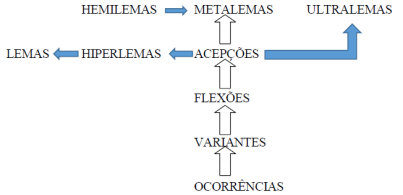
\includegraphics[width=.5\textwidth]{figuras/dado_hierarquia_delpo.png}
    \caption{Hierarquia de dados do DELPo}
    \label{fig:dados-hierarquia}
\end{figure}

Acima encontram-se termos criados com o único intuito de facilitar o tratamento
computacional dos dados a serem manipulados.

O \kw{Metalema} se trata de um conjunto de letras único e dotado de significado,
independente da quantidade de acepções a que corresponda. Não há metalemas iguais.
Isso o diferencia de um lema lexicográfico tradicional pois, como já mencionado,
uma palavra pode estar associado a um ou dois lemas.

Veja um exemplo: a palavra \say{manga} pode estar associada a dois lemas ($manga^1$--
fruta, $manga^2$--parte do vestuário). No entanto, não é possível para o moedor do
DELPo separar esses caracteres em dois lemas distintos, dado que o programa deveria
associar os devidos significados a cada palavra automaticamente. Para o sistema, a
fruta e a peça do vestuário são classificadas como um único metalema. A atribuição
de sentido aos verbetes, por outro lado, deve ser feita posteriormente por um
pesquisador.

Para acharmos o metalema de uma palavra adota-se a mesma metodologia que a lexicografia
tradicional adota para o lema. Ou seja, um metalema
\begin{itemize}
    \item de um verbo é sua forma no infinitivo (cantava \dir cantar)
    \item de um substantivo é sua forma no singular (mesas \dir mesa)
    \item de um adjetivo é sua forma no masculino singular (bonitas \dir bonito)
    \item é sempre adotado em sua ortografia atual (heróico \dir heroico)
\end{itemize}

\kw{Hemilema} é uma palavra que precisa da interpretação da acepção de um metalema para ser
compreendida. É a denominação usada ao tratar de abreviaturas e palavras truncadas devido a
fatores tais quais o mau estado de conservação das obras.

Tomemos, como exemplo, \texttt{mtos} e \texttt{mta}. Ambas são interpretadas como uma das
acepções do metalema \texttt{muito} e portanto não remetem a \texttt{muitos} e \texttt{muita},
suas respectivas flexões.

Convém observar que uma sigla, ainda que se trate de um tipo singular de abreviatura, será
tratada como metalema ao invés de um hemilema. Isso acontece pois há siglas que se assemalham
a nomes comuns\footnote{Crea, por exemplo} e só um pesquisador conseguiria classificá-las
da forma apropriada.

O conceito de \kw{Hiperlema} foi criado com a finalidade de recuperar as condições de homonímia
e polissemia, ausentes na constituição do metalema. Para que entendamos melhor como o conceito
de hiperlema é aplicado, é necessário definir alguns termos referentes às acepções.

Uma acepção é subordinada se remete a uma outra acepção, chamada subordinante. Se uma acepção
subordinante não for ao mesmo tempo subordinada, ela é chamada de acepção principal. Toda
acepção principal gera um hiperlema. Um metalema, por sua vez, pode ter duas ou mais acepções
principais e, nesse caso, gerará hiperlemas homônimos, o que nos possibilita fazer a distinção
entre homonímia e polissemia de um único metalema.\footnote{Porque precisamos de um hiperlema,
então? -- Notas de Estudante}

\kw{Ultralema} é um conceito pensado para tratar radicais, raízes e elementos de formação de
uma palavra (como prefixos e sufixos). A palavra \texttt{caligrafia}, por exemplo, possui dois
radicais (\emph{cali} e \kw{grafia}) e, portanto, dois ultralemas – um para cada radical. Já
a palavra \kw{bigamia} tem um prefixo \texttt{bi-}, e um radical \texttt{gamia}, e portanto,
também possui dois ultralemas – um para o prefixo e outro para o radical. Eis as formas de um
ultralema:
\begin{description}
    \item[\texttt{-x}] quando é um sufixo final
    \item[\texttt{-x-}] quando é um sufixo não final (requer uma vogal temática, por
    exemplo)
    \item[\texttt{x-}] quando é um prefixo
    \item[\texttt{x}] sem os hifens, nos demais casos (quando é raiz, por exemplo)
\end{description}

\section{O Back-end}
\label{sec:back-end}

Antes de entrar no mérito da definição de back e front end, é conveniente explicar o porquê da
separação dos tópicos. Além da óbvia separação entre os dois repositórios, deve-se pelo fato de
constituírem diferentes camadas do mesmo sistemas. Camadas distintas, desenvolvidas de outras
maneiras e com ferramentas distintas.

O back end, a camada mais funda do portal, é onde os dados são inseridos, consultados e removidos.
Esta camada, ao contrário da outra, não fica acessível ao cliente, que dificilmente compreenderia
o que está se passando.

\subsection{Ruby}
\label{subsec:ruby}

Ruby é uma linguagem de programação orientada a objetos criada por Yukihiro
Matsumoto em 1993. Ruby pode ser considerada um encontro entre Python,
Perl e Smalltalk. Por ser uma linguagem tão versátil e permitir que o
desenvolvedor concentre melhor suas energias em fazer o algoritmo\footnote{ao
invés de ficar lutando contra a programação}  como disseram \citet{Rcook:09}, e
pelos motivos citados abaixo, escolheu-se Ruby para o desenvolvimento do back end.

Ruby apresenta uma notável facilidade em lidar com expressões regulares
e com texto, fator de grave importância para a produção do moedor (funcionalidade
principal do sistema). Além disso, programar em Ruby é um exercício menos cansativo
do que com boa parte das outras linguagens, muito em razão de alguns de seus métodos
ou palavras chaves tornarem o texto do arquivo fonte mais compreensível para
humanos e máquinas exercitando a sugestão de D. E. Knuth que recomenda que a
programação deva ser feita de modo que humanos entendam o que se pediu da máquina.

Um arquivo bem formatado em Ruby permite que tal recomendação seja posta em
prática. Veja, na figura \ref{fig:ruby} um exemplo tirado do módulo auxiliar de
\texttt{autorias} (Entidade intermediária entre autor e obra\footnote{muitos para
muitos}). Além da obra de \citet{Rcook:09}, o site
\href{https://www.tutorialspoint.com/ruby/index.htm}{\textbf{Tutorials Point}}
também é uma boa sugestão quando se precisa de alguma ideia, ou em momento de dúvida.

O livro, tal como o título e os próprios autores \citet[xvii]{Rcook:09} sugerem, é um
livro de receitas. Apresenta soluções para problemas comuns e pequenos tutoriais. A
página, como o nome diz, é um compilado de tutoriais e é perfeito para quando há
dúvidas pontuais.

Quando a pesquisa visa compreender os limites do Ruby e do Rails, olhar a documentação
oficial é a melhor solução. Por se tratar de múltiplas páginas, não achei conveniente
colocar todas na bibliografia, senão o guia do Rails. No entanto, uma pesquisa com as
palavras chave \say{ruby}, o nome da classe a explorar e \say{docs} ajudam muito, também.
Pesquisar por gemas pra fazer algo no lugar do programador também gera bons resultados, sem
mencionar o tempo e energia poupados. Um bom exemplo é a gema que transforma números romanos
em decimais e vice-versa.

\begin{figure}
    \centering
    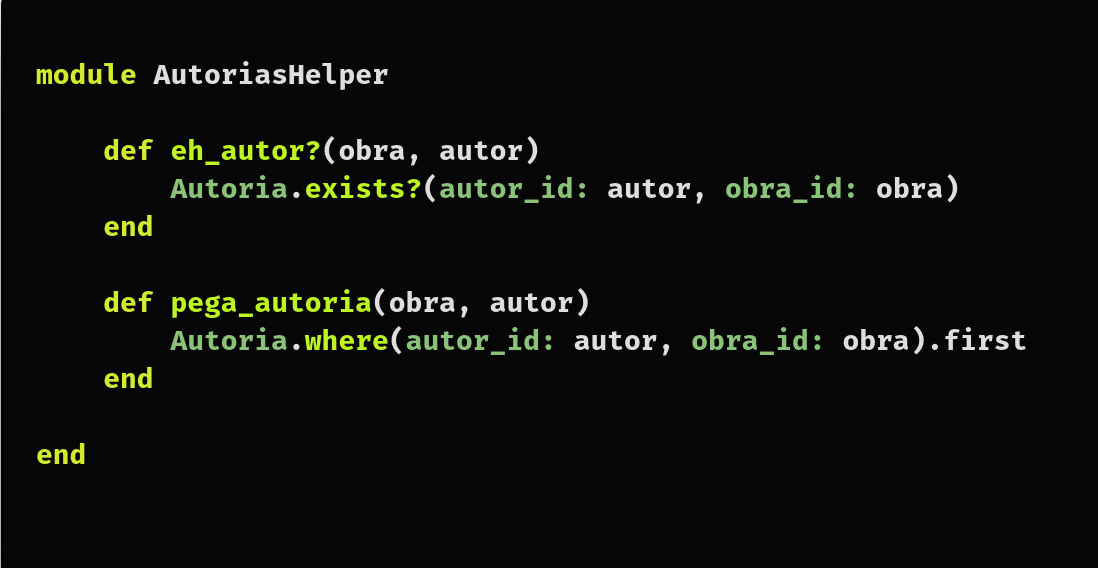
\includegraphics[width=10cm]{figuras/ruby}
    \caption{Consegue entender o que está sendo feito?}
    \label{fig:ruby}
\end{figure}

\subsection{Rails}
\label{subsec:rails}

Segundo \citet[p.~613]{Rcook:09}, \citetalias{RoR} (ou só Rails) é o que há de melhor
no universo Ruby, e ainda que ele não reinvente a roda em algum aspecto (utilizando-se
do que já foi verificado e validado como o próprio Active Record\footnote{responsável
por mapear os objetos criados no código em modelos e relacionamentos} e o paradigma MVC
-- Model, View, Controller).

Sobre o primeiro, convém saber que é o maior, senão o único responsável por \say{proteger}
o desenvolvedor de dores de cabeça com scripts de migrações e pesquisas e views nos
bancos de dados. Não que o desenvolvedor não possa colocá-las ali, mas dificilmente
há uma pesquisa que não se possa fazer sem a sua
\href{https://guides.rubyonrails.org/active_record_querying.html}{interface de busca}.
É um grande exemplo do que foi dito no início da sub-seção \ref{subsec:ruby} sobre
preocupar-se mais com o algoritmo a ser desenvolvido que com a linguagem em si.

O paradigma MVC é o conceito principal ao se tratar de Rails, ainda que não seja exclusivo
de ferramenta alguma, podendo mesmo ser aplicado a sistemas heterogêneos (leia-se que
utilizam mais de um framework). A sigla junta as iniciais das palavras \emph{model},
\emph{view} e \emph{controller}.
\begin{description}
    \item[model] relaciona os dados, cuida das validações a nível de back end, transações
    e buscas. O sistema conta com o \emph{ActiveRecord}, que serve de ponte entre o
    programador, além de gerar métodos de recepção de dados (\emph{getters}) e de manipulação
    (\emph{setters}) de acordo com os campos da tabela (figura \ref{fig:mvc}).
    \item[view] é a camada de visualização do Rails. Implementado com a biblioteca
    \emph{ActionView}, um sistema baseado em ERb\footnote{Embedded Ruby} para apresentar as
    views.
    \item[controller] fica no meio dos dois anteriores, e também é responsável por lidar com
    as requisições. De um lado, pega os dados necessários, de outro, organiza-os e manda para as
    views. É responsabilidade do \emph{ActiveController}
\end{description}

\begin{figure}[htb]
    \centering
    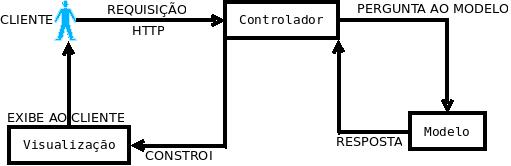
\includegraphics[width=.7\textwidth]{figuras/mvc.jpeg}
    \caption{Como funciona uma aplicação MVC (baseado no diagrama \href{https://blog.cloudboost.io/what-is-model-view-controller-124a9942246}{neste link})}
    \label{fig:mvc}
\end{figure}

Outro ponto muito forte (e ao mesmo tempo, um calcanhar de aquiles\footnote{chegarei aí ao falar
do front end}) da ferramenta são as convenções que, para o desenvolvedor tradicional de Rails,
importam mais que um arquivo de configurações gigante. Seguindo os padrões que a ferramenta estipula
também salva ao desenvolvedor muito tempo que pode ser usado para a criação e planejamento de novas
funcionalidades.

O \say{ponto de máximo} do Rails, seu grande destaque, vai para o desenvolvimento de aplicações que façam
CRUD (create, read, update e delete) de modelos em geral. Começa-se com um modelo conceitual em mente,
e pouquíssimo tempo depois há um produto mínimo viável. Ideal quando se deseja fazer determinada coisa
a toque de caixa.

Atualmente, vem sendo usado bastante no modo API (modo escolhido para esta aplicação). Usar esse
modo significa que sua aplicação serve JSON (Javascript Object Notation) ao invés de HTML. Além
disso, a aplicação em modo API (não só em Rails, como qualquer outra linguagem e framework) permite
que as respostas sejam coletadas por várias outras aplicações, e essa é só uma das vantagens de usar
o Rails desta forma. O \href{https://edgeguides.rubyonrails.org/api_app.html}{guia do modo API}
fornece algumas outras como a proteção a ataques como o de IP Spoofing.

\subsection{RSpec}
\label{subsec:rspec}

Provar que um método funciona $100\%$ das vezes requer, por vezes, uma prova
formal. Testes, de qualquer natureza (seja de integração ou unitário), têm como
finalidade garantir que o método vai dar a resposta correta nos cenários apontados.

Vale dizer também, que em um sistema robusto e cheio de funcionalidades, provar
formalmente que tudo está em perfeito estado é um trabalho hercúleo e cansativo
sem contar que é um grande redutor de produtividade. É por isso que se faz
necessária a construção de testes. Praticamente todo aluno de computação passou
por dificuldades ao caçar problemas em trabalhos no início de sua graduação.
Estes provavelmente saberão melhor o quanto convém ter um conjunto de testes
para as funções criadas.

Para produzir os testes que garantem, na medida do possível, a consistência e o
funcionamento completo do portal, esse projeto conta com RSpec. Diferentemente de
outras ferramentas de teste, o seu foco é no comportamento das funções\footnote{
BDD -- Behavior Driven Development} como podemos observar na figura \ref{fig:rspec}.
Trata-se da ferramenta mais adequada para garantir que os métodos e requisições a
serem desenvolvidos seguirão o comportamento esperado.

\begin{figure}[htb]
    \centering
    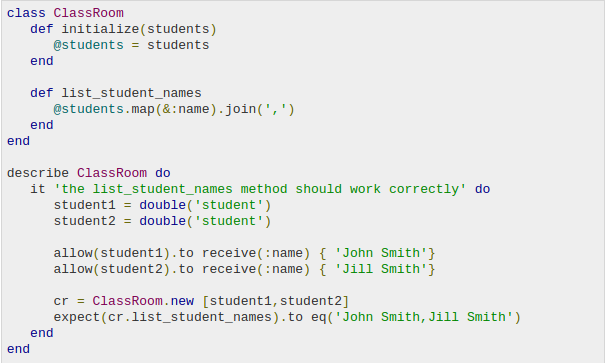
\includegraphics[width=10cm]{figuras/rspec}
    \caption{\label{fig:rspec} Exemplo de programa e teste respectivo}
\end{figure}

\section{O Front-end}
\label{sec:front-end}

Como mencionado na seção \ref{subsec:rails}, há um ponto negativo no Rails relativo à
\say{filosofia} do Rails em adotar muitas convenções. Se por um lado isso realmente facilita
a vida do programador, por outro lado, pode impossibilitá-lo de fazer determinadas coisas.
Em outras palavras, pode-se dizer que a experiência de usar Rails é boa quando se seguem os 
padrões, mas pode virar uma dor de cabeça ao tentar algo que foge muito aos padrões da ferramenta.

Por exemplo: não seria impossível usar algum framework Javascript para as views do Rails, mas
o trabalho necessário para produzir uma solução adequada é muito maior que usar o Rails como
API com uma aplicação em Nuxt.JS a parte.

\subsection{Vue JS}\label{subsec:vue-js}

Segundo o guia oficial, Vue (pronunciado como $/vju/$ \dir \textbf{view}), é uma ferramenta
voltada à produção de interfaces de usuário, sendo este o seu foco. No vídeo exibido na página
principal do \citetalias{Vue}, podemos ver alguns de seus traços básicos.

O principal ponto forte é a versatilidade. Mas em que sentido? A depender do que se precisa do
Vue, há uma receita do que pode ser feito. Quer fazer um site estático? É possível. Quer uma 
ferramenta que complemente um back end (produzindo uma produção fullstack)? Dá pra fazer, também. 
Vue é uma \say{massinha de modelar} com a qual se pode fazer bastante coisa.

Vue também é uma ferramenta acessível. Além de se tratar de um projeto de software livre, qualquer
desenvolvedor que tiver um bom domínio de HTML, CSS e JS pode utilizá-lo. Além disso, o programador
que está entrando em uma equipe utilizando Vue provavelmente terá pouco trabalho em se inteirar do
que foi feito. A curva de aprendizado pode ser suave, também.

Além disso, conta com uma grande quantidade de ferramentas afins construídas a partir dessa. Um
exemplo disso é o \href{https://www.youtube.com/watch?v=lIv1ItUzktc}{\textbf{VuePress}}, uma
ferramenta voltada à produção de documentação. Essa ferramenta compila arquivos em \emph{Markdown}
e os transforma em uma SPA (Single Page Application)

A figura \ref{fig:vue-example} mostra um componente Vue. Observe a separação clara do que é HTML e
o que é Javascript. Abaixo da tag template (HTML) e script (JS), há uma tag style (CSS) que pode ser
aplicada somente àquele componente ou não.

\begin{figure}[htb]
    \centering
    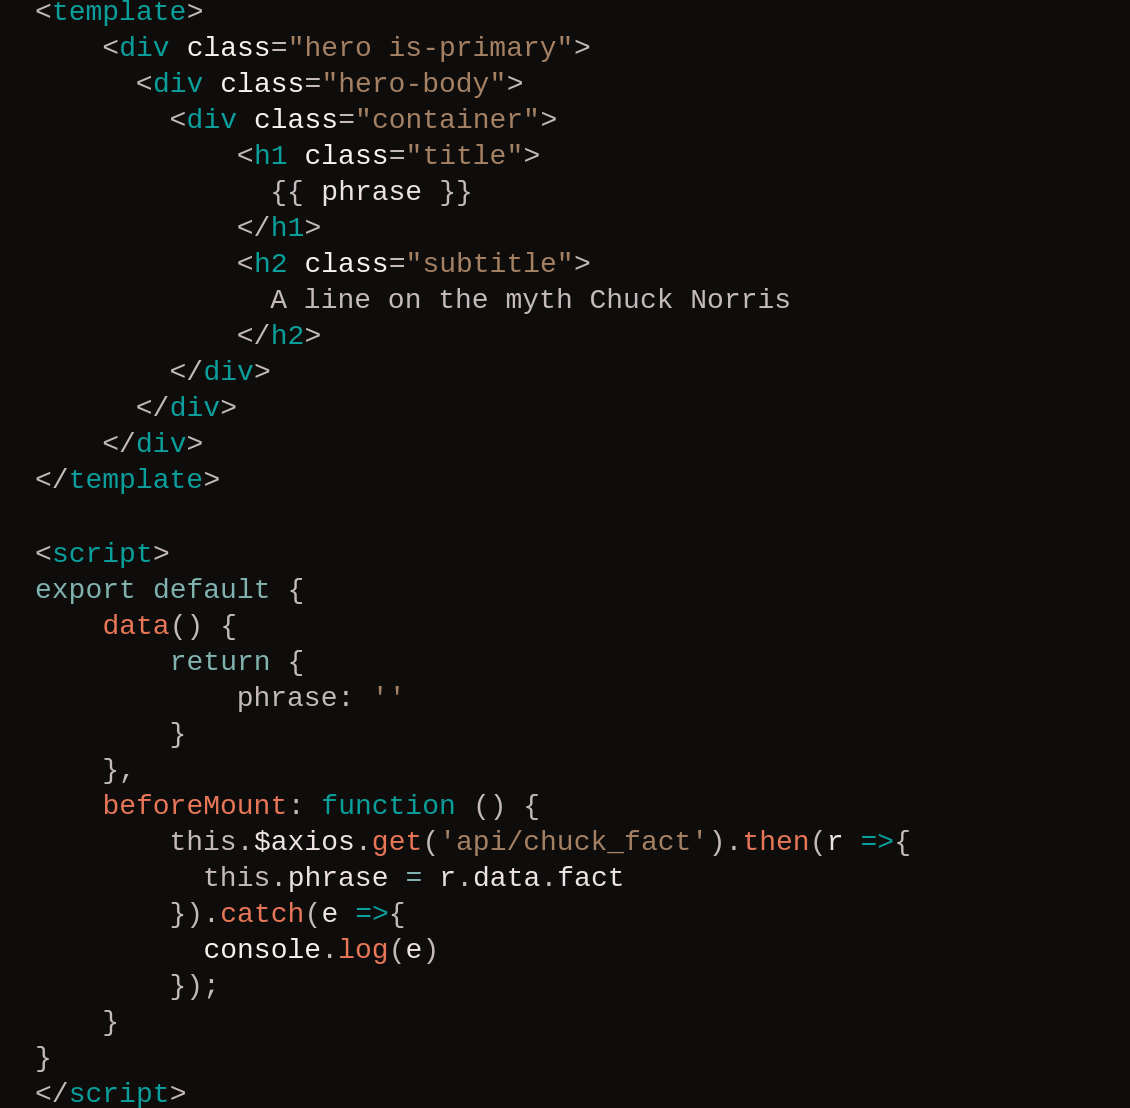
\includegraphics[width=.7\textwidth]{figuras/vue_template.png}
    \caption{Exemplo de um componente Vue}
    \label{fig:vue-example}
\end{figure}

\subsection[Nuxt JS]{Nuxt JS -- Vue on Steroids}\label{subsec:nuxt-js}

Baseado em seu guia oficial (está na bibliografia), Nuxt é um framework progressivo (ou seja, que
pode servir como uma biblioteca javascript ou framework) baseado em Vue.js. Seu foco é o mesmo que
o anterior, mas conta, por padrão, com muitas das bibliotecas que o desenvolvedor deve inserir 
manualmente no Vue. Esse é o motivo de dizer que Nuxt.js é um Vue com esteroides.

Longe de ser apenas uma versão fortificada do framework acima, Nuxt adota soluções para alguns
problemas comuns. Veja alguns desses.

Construir uma aplicação do zero não é trivial, e por isso talvez existam frameworks a facilitar tal
tarefa. Vue.js é um bom exemplo, e facilita muito a vida do desenvolvedor. Entretanto, não é tão
prático dado que a instalação inicial não inclui peças importantes como o
\href{https://vuex.vuejs.org/}{\textbf{Vuex}} e \href{https://router.vuejs.org/}{\textbf{Vue Router}}.
Não é difícil incluí-las, mas é bem melhor quando elas estão pré-instaladas e configuradas,
como vê-se implementado no Nuxt. Vale saber que muitas, senão todas as suas configurações padrão, são
baseadas no que os desenvolvedores consideram boas práticas.

Outra mudança notável é a organização das pastas e arquivos (veja a figura \ref{fig:file-system})

\begin{figure}[htb]
    \centering
    \subfloat[Vue]{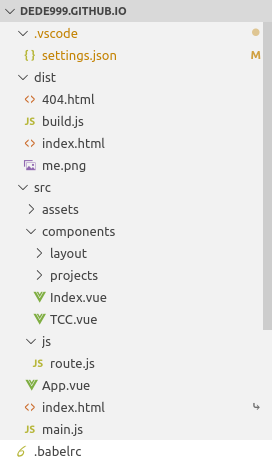
\includegraphics[width=.3\textwidth]{figuras/vue_dirs.png}}
    \subfloat[Nuxt]{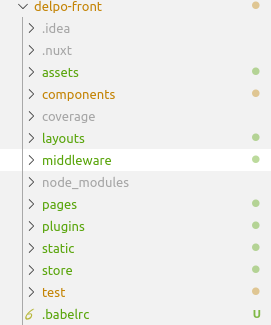
\includegraphics[width=.42\textwidth]{figuras/nuxt-dirs.png}}
    \caption{Organização de pastas e arquivos}
    \label{fig:file-system}
\end{figure}

Em projetos Vue (a), temos, por padrão, somente o diretório \texttt{src/} concentrando a maior parte
dos arquivos relevantes do projeto. Dentro deste, há uma separação maior, mas ainda não dá pra saber
que componentes gerarão páginas e quais serão simples componentes que as formarão. No Nuxt (b), não
há uma pasta que concentre quase todo o código da aplicação. Ao invés disso, há muitas pastas que
abrigam códigos cuja natureza está descrita pelo nome do diretório.

\emph{Search Engine Optimization}(SEO) é a propriedade de uma aplicação que facilita a  indexação e
pesquisa de elementos nela presente. Isso pode ser feito em Vue, por exemplo. A solução não é
difícil, mas envolve carregar página por página no servidor. Em uma plataforma menor talvez seja
viável. Entretanto, quando o sistema ganha em complexidade e capilaridade, torna-se cada vez menos
produtivo. O Nuxt é pré configurado para fazer isso sem que o desenvolvedor perceba, simplificando o
seu trabalho.

Quando uma aplicação Vue.js é carregada no servidor, o processo leva um pouco mais de tempo na primeira
vez se comparado aos posteriores recarregamentos que sobem somente as mudanças feitas. Isso acontece
porque toda a aplicação é carregada ao mesmo tempo nesta ocasião. No caso do Nuxt, só o HTML e o CSS
são pré-carregados por padrão. O javascript é carregado por demanda, e isso permite que o carregamento
das páginas ocorra de maneira mais rápida.

Para finalizar, vale mencionar duas características deste framework:
\begin{itemize}
    \item Ao contrário de seu predecessor, Nuxt é mais fácil de configurar, e permite que as configurações
    padrão sejam sobrescritas com menos trabalho.
    \item Configura rotas de acordo com a organização do arquivos no diretório \texttt{pages/}.
\end{itemize}

\subsection{Jest}\label{subsec:jest}

\citetalias{Jest}, de modo similar a RSpec, é uma ferramenta de testes para Javascript criada pela equipe do Fecebook,
motivo pelo qual alguns acreditam que seja uma biblioteca exclusiva do React (framework javascript também
desenvolvida pelo Facebook), o que não é verdade.

É uma ferramenta com um ótimo desempenho de execução, e isto se deve parcialmente ao fato de que cada teste
é rodado num processo distinto rodando em paralelo com os demais. Isso é possível, pois cada teste tem o seu
\say{contexto global} garantindo independência entre cada um. Para aumentar ainda mais a performance, testes
que falharam são executados primeiro. Além disso, os testes são organizados baseado no tempo necessário a
executá-los.

A ferramenta verifica a cobertura de testes na aplicação. Em outras palavras, inserindo um argumento de linha
de comando\footnote{Em aplicações Nuxt, essa verificação é feita sem a necessidade de argumentos adicionais}
\texttt{\kw{- -coverage}}, é possível que se veja o quanto de cada parte do código é verificado através dos
testes. Pode-se questionar a importância dessa funcionalidade. Entretanto, saber o que já foi coberto é
importantíssimo para dirigir os esforços na direção certa. Importante saber que a cobertura de testes será
exibida na sessão \ref{subsec:testes-cobertura} do capítulo dos resultados obtidos.

Outras características bem interessantes do Jest:
\begin{description}
    \item[boas falhas] Jest provém o desenvolvedor com mensagens significativas a cerca do motivo daquele teste
    ter falhado, o que é crucial para eliminar o erro.
    \item[configurações] Jest pode rodar com pouca ou nenhuma configuração.
    \item[mocking] com Jest, é possível simular qualquer objeto fora do escopo do teste.
\end{description}

\begin{figure}[htb]
    \centering
    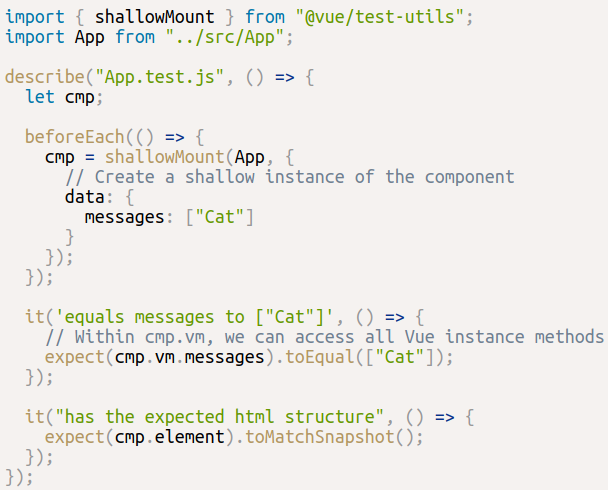
\includegraphics[width=.55\textwidth]{figuras/jest.png}
    \caption{Exemplo de um conjunto de testes usando Jest}
    \label{fig:jest}
\end{figure}

\section{Boas práticas em programação}
\label{sec:boas-praticas}

Na sesão \ref{sec:goals}, falou-se da importância de um código limpo. Aqui tratar-se-á de como produzir código
de qualidade. Para isso foi trazido uma publicação de \cite{BP} que cita práticas que enriquecem a qualidade do
código. Aqui são mencionados os pontos mais importantes.

\subsection{SOLID}\label{subsec:solid}

SOLID é uma sigla formada pelo título de cada um dos 5 princípios.
\begin{description}
    \item[S] Single Responsibility Principle \dir Cada classe ou função deve ter uma responsabilidade única no
    sistema -- O importante é que classes e funções tenham uma tarefa
    \item[O] Open-closed Principle \dir Objetos e entidades devem ser abertos a extensão, e fechados a modificação
    -- Em outras palavras, sempre que algo novo precisar ser criado, o correto é criar uma função nova, e não
    alterar o que já foi feito.
    \item[L] Liskov Substitution Principle \dir Se a classe B herda da classe A, então você deve ser capaz de usar
    B no lugar de A sem quebrar a funcionalidade -- Dado que haja uma classe \textbf{\texttt{Animais}} que possua
    um método \textbf{\texttt{andar}} que retorne as novas coordenadas do bicho. Se houver uma outra classe
    \textbf{\texttt{Felinos}} que herde da primeira, e que esta também possua o método \textbf{\texttt{andar}}.
    Neste caso, o método deve retornar a mesma coisa, ou seja, as novas coordenadas do felino.
    \item[I] Interface Segregation Principle \dir Desenvolvedores não devem implementar métodos de interface que
    não vá usar -- Se há métodos que uma interface não utiliza, ela tem que ser quebrada em mais.
    \item[D] Dependency Inversion \dir Abstrações não devem depender de detalhes. Detalhes devem depender de
    abstrações -- Uma classe deve ser a mais abstrata possível, e não deve depender de outras classes
\end{description}


\subsection{Outras recomendações}\label{subsec:recomendacoes}

Além desses preceitos, há outros pilares a levar em conta, e quando seguidos, melhoram e muito a qualidade do
código.
Eis alguns desses presentes no texto de \cite{BP}
\begin{itemize}
    \item Use nome de variáveis que tenham significado e que sejam fáceis de pronunciar. Nomes como \texttt{\kw{i}},
    \texttt{\kw{x}} e \texttt{\kw{item}} são contra exemplos fortíssimos.
    \item Ainda sobre variáveis, é aconselhado que os nomes auto explicativos, de forma que comentários não sejam
    necessários. Ex: \texttt{\kw{SaveRecord}} \dir \texttt{\kw{SavePerson}}
    \item Faça uso extensivo de constantes. Ex: \texttt{\kw{if age >= 18}} \dir \texttt{\kw{if age >= LEGAL-AGE }}
    \item Evite funções com mais de um \texttt{if} encadeado.
    \item Evite código duplicado.
\end{itemize}

Há outros mais, e vale dizer que muitos desses pilares estão mencionados no texto de \cite{CCL}, como o que
se refere a nomes de variáveis.
Como já foi dito antes, dada a multiplicidade de diretrizes, não é trivial que todas sejam seguidas.
O importante é ter uma ampla noção sobre o que é um código de qualidade.